\chapterimage{/4/head.jpg} % Chapter heading image
\chapter{Cinque Problemi del Modello Standard}\label{4:ch}

Ci sono alcuni problemi radicati nel modello del Big Bang che vengono in parte risolti includento il fenomeno dell'inflazione.

\section{Problema dell'Origine (Big Bang)}
Il fenomeno del Big Bang è implicito nelle equazioni di Friedmann (relatività generale + spazio omogeneo e isotropo (RW) + fluido perfetto). Ossia assumendo l'andamento $a\propto t^\beta$, $\ddot{a}<0$ e $\dot{a}_0 >0$ come osservato, la funzione monotona crescente $a(t)$ prima o poi deve sbattere sull'asse y.   
Il Big Bang è però matematicamente molto brutto perché per $t\rightarrow 0$ si ha $\rho \rightarrow \infty$, $H \rightarrow \infty$ e $T \rightarrow \infty$, questo può essere evitato in 3 modi:
\vspace{0.5em}
\begin{enumerate}
    \item Ponendo $\ddot{a}>0$ (flesso) $\Leftrightarrow w<-1/3$. Nella fisica ordinaria questo non è possibile ed è quindi necessario introdurre la costante cosmologica. Tuttavia, le misurazioni della costante cosmologica vincolano il flesso a tempi tardi, lontano dal Big Bang. É quindi necessario introdurre un'ulteriore componente sconosciuta che generi un flesso vicino al Big Bang ($@ \_ @$).
    \item Abbandonando l'ipotesi di fluido perfetto includendo effetti di viscosità (bulk $\xi$ e shear $\eta$) e di conduzione. Le equazioni di Eulero nel primo caso diventano: $$ \rho \left ( \frac{\partial v}{\partial t} + (v \cdot\nabla)v \right )= -\nabla p +\eta \nabla^2v + \left ( \xi + \frac{\eta}{3} \right )\nabla(\nabla\cdot v). $$ Si può dimostrare che l'introduzione della shear viscosity o della conduzione porterebbero alla violazione di omogeneità e isotropia.
    \item Abbandonando l'ipotesi di omogeneità e isotropia (modelli di Bianchi).
\end{enumerate}

Si preferisce da un punto di vista pratico rimanere nella condizione di avere omogeneità e isotropia, pur dovendo affrontare il problema di giustificare la singolarità.

\subsection{Scala di Planck}
Sfruttando dimensionalmente il principio di indeterminazione di Heisemberg:
$$
\Delta E \Delta t \leq \hslash \quad \rightarrow \quad (G t_P^2)^{-1} (c t_P)^{3}c^2 t_P \approx \hslash \quad \rightarrow \quad t_P \approx \sqrt{\frac{\hslash G}{c^5}} \approx 10^{-43}~\mathrm{s}
$$
Per $t<t_P$ è necessario quantizzare la gravità, problema ancora aperto. La trattazione che segue sarà quindi svolta a partire dal tempo di Plank. Alcune quantità fondamentali legate questo istante sono:
\begin{equation}\left\{
    \def\arraystretch{1.5}
        \begin{array}{ll}
        T_P \simeq 10^{32}~\mathrm{K} \\
        E_P \simeq 10^{19}~\mathrm{Gev} \\
        n_P \simeq 10^{98}~\mathrm{cm}^{-3} \\
        m_P \simeq 10^{-5}~\mathrm{g} \\
        \rho_P \simeq 10^{93}~\mathrm{g\: cm}^{-3}  \\
        l_P \simeq 10^{-33}~\mathrm{cm} \\
        \sigma = (entropia) = 1 
    \end{array}\right. \label{eq:unitaplanckiane}
\end{equation}
Il valore unitario dell'entropia simula la presenza di una sola particella (1 g.d.l.), sarà quindi necessario ad un certo momento trovare un meccanismo fisico in grado di creare particelle.  

\subsubsection{Tempo di Compton}
É il l'intervallo di tempo (o lunghezza) sopra al quale possiamo ignorare gli effetti quantistici:
\begin{equation}
    t_C = \frac{\hslash}{mc^2} \quad \rightarrow \quad l_C =  \frac{\hslash}{mc}
\end{equation}

\subsubsection{Tempo di Schwarzschild}
É la scala alla quale la velocità di fuga è pari alla velocità della luce:
\begin{equation}
    l_S =  \frac{2Gm}{c^2}  \quad \rightarrow \quad   t_S = \frac{2Gm}{c^3} 
\end{equation}


\subsubsection{Tempo di Planck}
É il momento in cui la scala di Schwarzschild corrisponde alla scala Compton $t_C(m_P)=t_S(m_P)$ e da questa uguaglianza si definisce la massa di Planck. In altre parole: il tempo che descrive la gravità è esattamente uguale al tempo che descrive gli effetti quantistici, per le fasi successive si può ignorare la meccanica quantistica.

L'energia emessa da un buco nero dipende dalla sua temperatura (legata alla \textbf{radiazione di Hawking}) , $T=10^{-7} (M/\msun)^{-1}$ K. Il tempo tipico di evaporazione di un buco nero vale: $\tau_{evap}=10^{10} (M/10^{15}~\textrm{g})^{3} $ yr. Si può calcolare che il tempo di evaporarione di un buco nero di massa pari alla massa di Planck vale esattamente $t_P$. Questo apre la possibilità di pensare che prima del tempo di Planck vi fosse un continuo emergere ed evaporare di buchi neri nessuno dei quali poteva sopravvivere. A causa di una fluttuazione quantistica, uno di questi buchi neri è sopravvissuto per un tempo maggiore di $t_P$ ed è diventato il nostro universo. Questo è una delle possibilità adottate nei modelli per evitare il problema della singolarità. 





\section{Problema dell'Orizzonte}
Assumendo $a\propto t^\beta$ si può osservare che il raggio dell'orizzonte (\ref{eq:raggioriz}) non diverge solo per $\beta < 1$. La divergenza implica che tutto l'universo sia in connessione causale. Inoltre, confrontando $\ddot{a}\propto \beta (\beta-1) ~t^{-2} ~a $ con la prima equazione di Friedmann, si ha che il Big Bang esiste, $\ddot{a} < 0 \Leftrightarrow 0 < \beta < 1$. La condizione per avere un Big Bang è necessariamente implicata dall'avere un orizzonte cosmologico. 

Il problema dell'orizzonte deriva dall'osservazione della quasi perfetta isotropia della CMB. Questo richiede che ci sia stata una connessione causale che ha consentito ai fotoni della CMB di mettersi in equilibrio, ossia questo processo deve essere avvenuto dentro l'orizzonte. Confrontando la scala dell'orizzonte con quella della CMB al momento dell'ultimo scattering (LS) fra fotoni ed elettroni ($z_{LS}\approx 10^3$):

\begin{equation*}
R_H = \frac{3(1+w)}{1+3w} ~c ~t_{LS} \approx  3 ~c ~t_0 ~ (1+z_{LS})^{-3/2} \qquad\qquad r_{LS} = \frac{c ~(t_0 - t_{LS})}{1+z_{LS}} \approx \frac{c ~t_0}{z_{LS}}
\end{equation*}

si ha la relazione: $R_H(z_{LS}) = 3 ~r_{LS} ~z_{LS}^{-1/2} \approx 0.1 ~r_{LS} $. Questo è in conflitto con l'osservabile (CMB), che deve essere stato prodotto in condizioni di connessione causale. Si cerca una soluzione matematico-grafica utilizzando un altro raggio, quello della sfera di Hubble ($\tilde{R}_H (t) = c/H $) che ha un valore pressoché equivalente al precedente nell'universo primordiale. Per graficare le soluzioni si utilizzano le quantità riscalate a meno dell'espansione, in particolare $\tilde{R}_H \rightarrow c ~a_0 / \dot{a}$ e si ha comunque $R_{H,c} \approx \tilde{R}_{H,c} $. 

Calcolandone la derivata si può notare che $\dot{R}_{H, c}=- c ~a_0 ~\ddot{a} / \dot{a}^2 \propto - \ddot{a}$. Per cui, nei modelli di Friedmann ($\ddot{a}<0$), il raggio della sfera di Hubble comovente $\tilde{R}_{H,c} (t)$ è una funzione monotona crescente. Data una scala qualsiasi, ad esempio $r_{LS}$, si può determinare il $t'$ in seguito al quale tale scala è completamente in connessione causale. 

\begin{figure}[h]
    \centering
    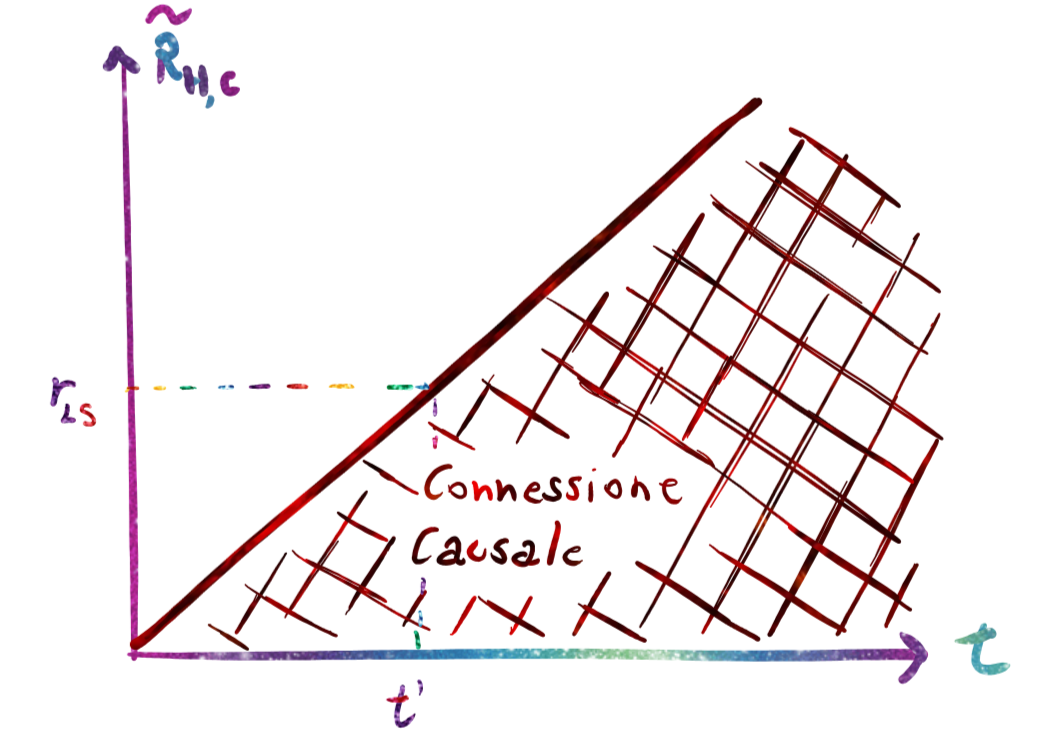
\includegraphics[width=.8\textwidth]{Pictures/4/rsferahubble-t.png}
    \caption{Andamento della Temperatura di materia e radiazione pre e post disaccoppiamento.}
    \label{fig:4}
\end{figure}

Il problema può essere risolto assumendo che esista un periodo in cui la curva diventa monotona decrescente tra un $t_i$ e un $t_f$ (\textbf{periodo inflazionario}). In questo modo può esistere un intervallo entro il quale una data scala è stata in connessione causale, in questo periodo l'universo ha avuto modo di raggiungere l'equilibrio termico anche se oggi osservo che questa scala è fuori dall'orizzonte. Nel periodo inflazionario è necessario avere $\dot{R}_{H, c}<0 \rightarrow \ddot{a}>0  \rightarrow w <-1/3$ per un periodo sufficiententemente lungo. Passando a coordinate comoventi si è fattorizzata via l'espansione dell'universo, per questo il raggio dell'orizzonte comovente può decrescere.


\begin{figure}[h]
    \centering
    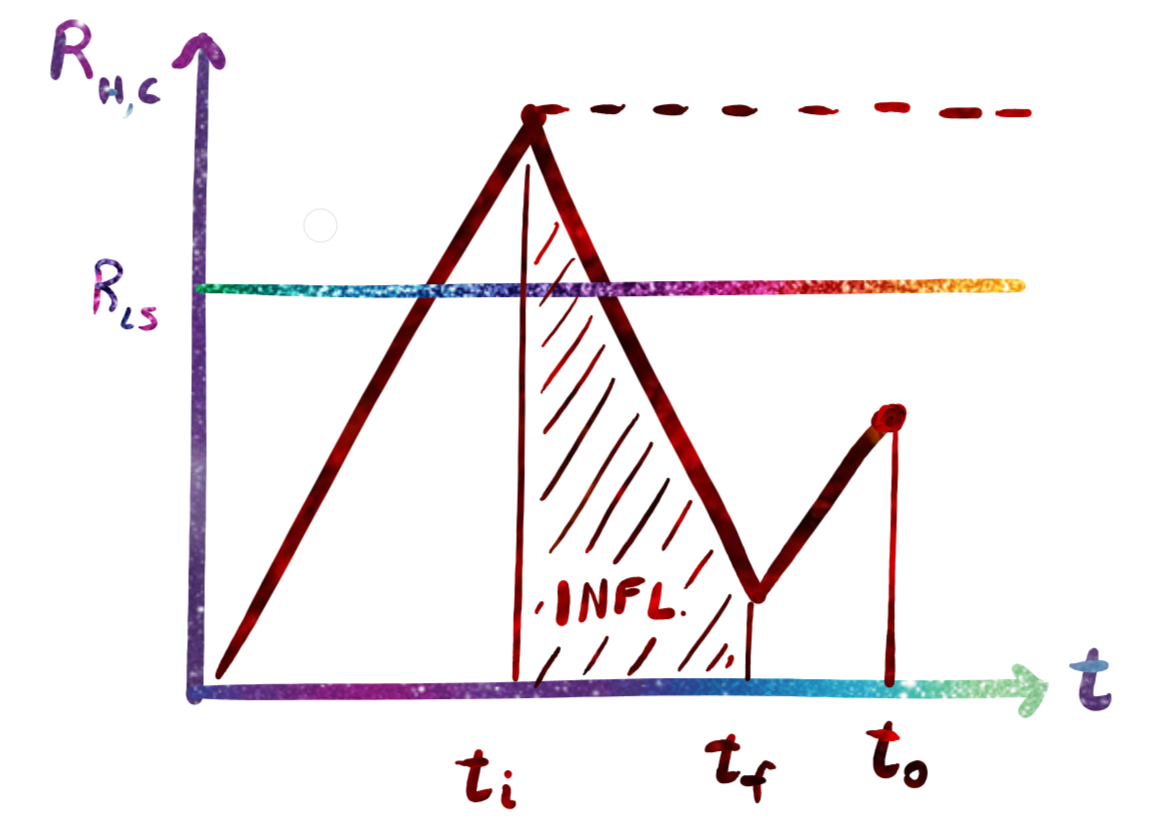
\includegraphics[width=.6\textwidth]{Pictures/4/pbhorsol.png}
    \caption{Soluzione al problema dell'orizzonte. $R_ {LS}$ è il raggio della scala al momento dell'ultimo scattering.}
    \label{fig:4}
\end{figure}

Dall'equazione (\ref{eq:hevol}), assumendo $\Omega_0 = 1$ (universo primordiale) e definendo $s=3(1+w)/2$ si può ottenere integrando per separazione delle variabili:
\begin{equation}
    a(t)=a_i \left( 1+s(t-t_i) ~H(t_i)\right)^{1/s}
\end{equation}
Al variare del parametro $w$ si ha:
\begin{equation}
    a(t) \propto \left\{\begin{matrix}
        t^{1/s} & -1 < w \le 1/3\\ 
        (cost-t)^{1/s} & w<-1 \\
        \exp (t/\tau)&  w=-1
       \end{matrix}\right.
\end{equation}
Nei primi due casi l'espansione è a legge di potenza, nel terzo caso è esponenziale. Derivando la funzione $H(t)$ si può ricavare la relazione:
\begin{equation}
    \ddot{a}= a\dot{H} + \frac{\dot{a}^2}{a} = a \left(  \dot{H} + H^2\right)
\end{equation}
Per $\dot{H}>0$ si ha \textbf{superinflaizone} ($w<-1$), se $\dot{H}<0$ si ha \textbf{subinflaizone} ($-1 < w \le 1/3$), l'inflazione standard si ha per $\dot{H}=0$ ($w=-1$).

\subsubsection{Stima della durata dell'Inflazione}
La condizione è che la sfera di Hubble comovente all'inizio dell'inflazione $\tilde{R}_{H,c}(t_i)$ deve essere molto (per evitare problemi antropocentrici) più grande della sfera di Hubble oggi ${R}_{H,c}(t_0)$.
\begin{equation*}
\frac{c ~a_0}{H_i ~a_i} \gg \frac{c}{H_0} \quad \rightarrow \quad a_0 ~H_0 \gg a_i ~H_i
\end{equation*}

Attraverso l'equazione (\ref{eq:hevol}) si può esprimere come la relazione è variata nel tempo avendo cura di separare i periodi in base al prorpio $w$:
\begin{equation*}
\frac{a_i ~H_i}{a_f ~H_f}\quad ^{[w<- \frac{1}{3}]} \qquad\ll\qquad \frac{a_0 ~H_0}{a_f ~H_f}\quad = \quad\frac{a_0 ~H_0}{a_{eq} ~H_{eq}} \quad ^{[w=0]}\quad \times \quad\frac{a_{eq} ~H_{eq}}{a_f ~H_f} \quad ^{[w= \frac{1}{3}]}\quad
\end{equation*}
per cui:
\begin{equation}
    \left( \frac{a_f}{a_i}\right)^{-(1+3w)} \quad\gg\quad \frac{a_0}{a_{eq}} \left( \frac{a_{eq}}{a_f}\right)^2 \simeq 10^{60} ~z_{eq}^{-1} \left( \frac{T_f}{T_P}\right)^2
\end{equation}
Questo valore stabilisce di quanto deve essere variato il fattore di scala durante l'inflazione per risolvere il problema dell'orizzonte. La stessa variazione viene parametrizzata attraverso il cosiddetto \textbf{numero di e-folding} $N_{ef}=\ln (a_f/a_i)$:

\begin{equation}
    N_{ef} \gg \frac{60}{\left | 1+3w   \right |} \left(  2.3 + \frac{1}{30}\ln\frac{T_f}{T_P}-\frac{1}{60}\ln z_{eq}  \right) \quad \rightarrow \quad  N_{ef} \gg 60
\end{equation}
Questo corrisponde ad un aumento del volume dell'universo di $180$ dex.

\vspace{1em}
\noindent Morale, il problema dell'orizzonte è quindi risolto se:
\begin{itemize}
    \item Si assume che esiste un periodo in cui l'universo è in espansione accelerata;
    \item La durata di questo periodo è sufficiente per far sì che $N_{ef} \gg 60$;
    \item Si trova una giustificazione fisica per questa soluzione matematica.
\end{itemize}

\section{Problema dell'Età dell'Universo (o della Piattezza)}
La seconda equazione di Friedmann(\ref{eq:friedmann2}) è stata interpretata dal punto di vista newtoniano come l'equilibrio tra un termine cinetico e un temrine potenziale determinato dalla costante $k$. Nell'epoca primordiale (era radiativa) tutte le forze sono unificate e non ci sono scale privilegiate: l'unico tempo scala è il tempo di Planck. Ci si aspetterebbe quindi che: per un universo chiuso $2t_{max}\sim t_P$; per un universo aperto $t^* \sim t_P$ dove $t^*$ è il tempo oltre al quale la curvatura è trascurabile e $a\propto t$ asintoticamente. In questo secondo caso si può utilizzare la temperatura $T_R\propto a^{-1}$ per misuare l'età dell'universo attesa: $t_0 = t_P T_P / T_0\simeq 10^{-43+32-0}\simeq 10^{-11}$ s. La durata dell'universo palesemente maggiore dei due risultati ottenuti potrebbe quindi essere dovuta all'insolito fatto che fra tutti i valori possibili, valga esattamente $\Omega=1$ (universo piatto). 

In particolare, affinché valga $\Omega_0=1$, ai tempi di Planck ($w=1/3$) si doveva avere:
$$
    \Omega_P = 1+\frac{ \left| \Omega_0 -1 \right|}{\Omega_0(1+z_P)^2} = 1 + \left| \Omega_0 -1 \right|\cdot 10^{-60}
$$
Avere un valore così stringente nei modelli non è bello e viene definito \textbf{problema di fine-tuning}. Supponendo che il valore differisse anche poco dall'unità, $\Omega_P=1.01$, oggi si avrebbe $\Omega_0=10^{58}$ e già negli anni '70 ($\Omega_0\simeq 1 \pm 10$) i cosmologi non sarebbero stati contenti.

Attraverso l'equazione (\ref{eq:2omega0k}) si possono sviluppare le seguenti relazioni:
\begin{equation}
    H_0^2 \left ( 1-\Omega_0 \right ) = -\frac{kc^2}{a_0^2} \equiv \frac{a^2}{a_0^2} \left( H^2 - \frac{8}{3}\pi G \rho\right) \quad \rightarrow \quad \frac{a^2}{a_0^2} H^2 (1-\Omega) = cost
\end{equation}
dividendo la quantità costante per $T_0$ e moltiplicando per $(\hslash /k_B)^2$ per renderla adimensionale:
\begin{equation}
    |\varepsilon (t) | := |k| \left( \frac{\hslash c}{a k_B T}\right)^2 = \frac{H_0^2 |\Omega_0 -1|}{T_{0R}^2}\frac{\hslash^2}{k_B^2} \simeq | \Omega_0 -1 | \cdot 10^{-58} < 10^{-57}
\end{equation}
A questo punto si può porre a zero richiedendo $k=0$ per tutta la durata dell'universo. Questa quantità può essere legata all'entropia dell'universo (ossia della radiazione per l'universo primordiale):
\begin{equation}
    \sigma_u = \frac{S_R ~a^3}{k_B} \simeq \left( \frac{k_B Ta}{\hslash c} \right)^3 \simeq \varepsilon (t) ^{-3/2} > 10^{86}
\end{equation}
Un valore così elevato dell'entropia rispetto a quello del tempo di Planck ($\sigma=1$), richiede la creazione di un numero elevatissimo di particelle (che giustificherà la piattezza). 
Il problema può essere risolto assumendo che esista un intervallo di tempo durante il quale il valore di $\Omega$ si avvicini molto all'unità, contrariamente all'evoluzione predetta dai modelli di Friedmann. Affinché questo avvenga (cfr. eq. \ref{eq:2omega0k}) bisogna avere $w<-1/3$ (espansione accelerata, e.g. inflazione), di durata sufficiente. La condizione da imporre è $(1-\Omega_i^{-1})/(1-\Omega_0^{-1})\ge 1$, ossia $N_{ef}\ge 60$. Con la condizione del paragrafo precedente,  $N_{ef}\gg 60$, $\Omega$ si schiaccia ancora di più a 1 (nel caso in cui si misurasse $\Omega=0.98$ si butta via il modello).

\begin{figure}[h]
    \centering
    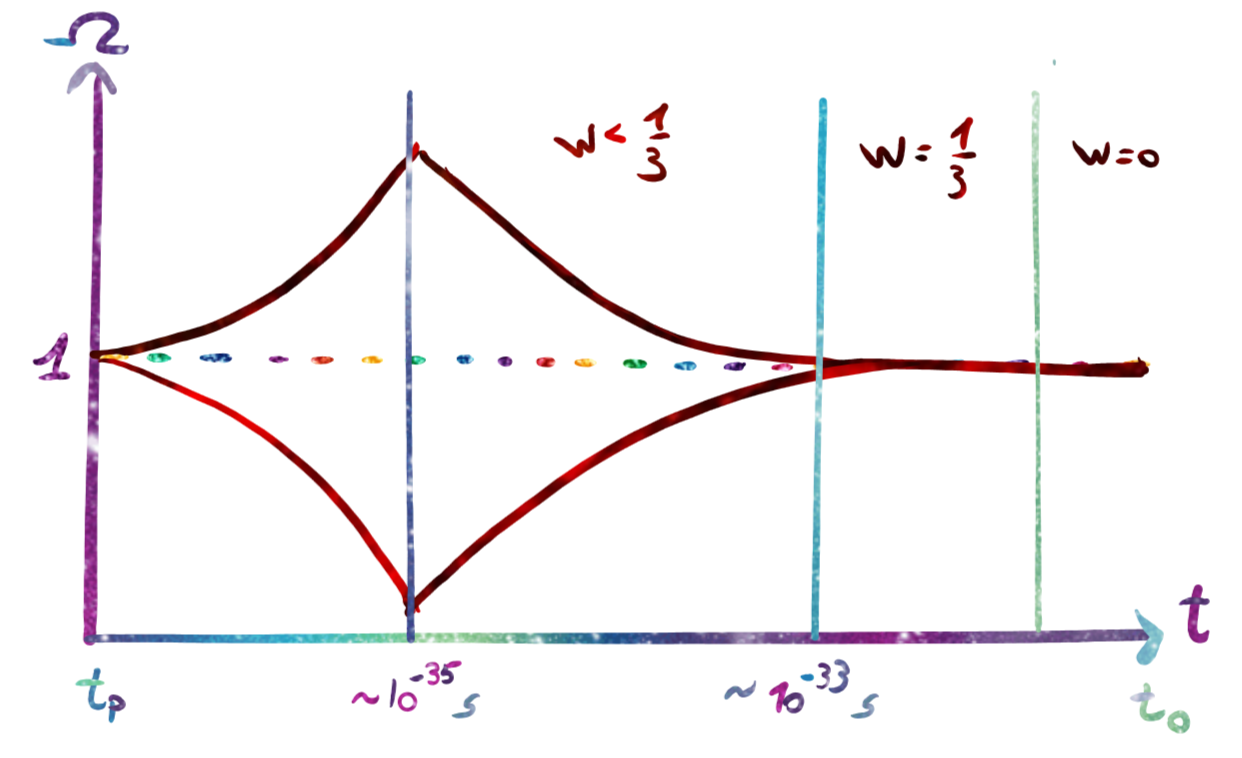
\includegraphics[width=.7\textwidth]{Pictures/4/omegainflation.png}
    \caption{Andamento della Temperatura di materia e radiazione pre e post disaccoppiamento.}
    \label{fig:4}
\end{figure}

\vspace{1em}
\noindent Morale, il problema dell'età (della piattezza) è quindi risolto se:
\begin{itemize}
    \item $N_{ef} \ge 60$ (condizione meno stringente della precedente);
    \item Si trova una giustificazione fisica per questa soluzione matematica.
\end{itemize}




\section{Problema dei Monopoli Magnetici}
In base alla Teoria della Grande Unificazione (GUT) esiste un tempo dell'universo prima del quale la forza elettrodebole e la forza forte erano unificate, inoltre ci si aspetta che come esistono le cariche fondamentali del campo elettrico, esistano anche quelle del campo magnetico (\textbf{monopoli magnetici}). Una carica fondamentale è espressa in unità di carica di Dirac:
\begin{equation*} 
    g_n = n g_0 \qquad g_0 = 68.5 e = \frac{\hslash c}{2e}
\end{equation*}
La massa che dovrebbe corrispondere ai monopoli magnetici è espressa in unità di masse corrispondenti all'energetica della transizione GUT ($m_{GUT}\simeq 10^{14\div 15}$ GeV):
\begin{equation*} 
    m_{MM}\simeq 10^2 ~m_{GUT} \simeq 10^{16}\; \mathrm{GeV}
\end{equation*}

La creazione dei monopoli magnetici deve avvenire all'interno dell'orizzonte, per cui si può stimare la loro densità: $n_{MM}(t_{GUT})\ge 10^{-10} ~n_\gamma(t_{GUT})$. Al momento non sono stati trovati processi fisici che possano variare il rapporto $n_{MM}/n_\gamma$ (simile a $n_b/n_\gamma$), ma ad oggi sono stati osservati 0 monopoli magnetici.

Inoltre il parametro di densità dei monopoli magnetici dovrebbe valere:
\begin{equation*}
    \Omega_{MM,\, 0} = \frac{n_{MM,\, 0} ~m_{MM}}{\rho_{cr,\, 0}} \approx \Omega_{0b}\frac{m_{MM}}{m_p}\approx \Omega_{0b} \cdot 10^{16}
\end{equation*}
e genererebbe quindi un universo chiusissimo.

\vspace{1em}
\noindent Morale, la teoria GUT per descrivere l'universo primodiale prevederebbe anche:
\begin{itemize}
    \item Una densità attuale di monopoli magnetici simile a quella dei barioni (vs. osservazioni);
    \item Un valore attuale di $\Omega_0$ esagerato.
\end{itemize}
Anche in questo caso l'inflazione potrebbe risolvere il problema diluendo sufficientemente i monopoli magnetici da renderli oggi insignificanti.

\section{Problema della Costante Cosmologica}
Osservando l'espansione accelerata dell'universo ($q_0=-0.55$) si ha un'evidenza passiva della costante cosmologica. Il problema fisico risiede nel fatto che, prendendo dalle osservazioni $\Omega_{0\Lambda}$, si ottiene un valore estremamente piccolo $\Lambda\simeq 10^{-55}$ cm$^{-2}$. La massa associata a tale campo sarebbe:
$$
m_\Lambda = \left( \frac{\rho_\Lambda ~\hslash^3}{c^3}\right)^{1/4} \le 10^{-32}\; \mathrm{eV}
$$
che è una quantità estremamente bassa. La costante cosmologica può essere interpretata come la densità del vuoto. Nel caso avvenga una transizione di fase, parte dell'energia del vuoto può essere estratta, in particolare $\Delta \rho_V \sim m^4 c^3 / \hslash^3$, per generare la nuova fase ordinata. FIGURAA.

\subsubsection{Energia del vuoto al tempo di Plank}
Si ottiene risommando tutta l'energia spesa nelle diverse transizioni di fase:
$$
\rho_V (t_P) = \rho_V (t_0) + \sum_{jumps} \frac{m_i^4}{(\hslash / c)^3}= \sum_{jumps} \left ( 1 + 10^{-108}\right)\; \mathrm{GeV^4}
$$
Anche in questo caso si è di fronte a un problema di fine-tuning, ossia il vuoto aveva moltissima di energia e ha perso $108$ ordini di grandezza che però non possono essere posti a $0$ altrimenti non ci sarebbe $\Lambda$ oggi. Inoltre ci si chiede come mai la costante cosmologica abbia un contributo non trascurabile solamente oggi e, per non essere antropocentrici, questo è un problema di coincidenza che può essere alleggerito con $w<-1/3\neq -1$ spostando indietro nel tempo il momento in cui $\rho_\Lambda=\rho_m$ (modelli di quintessenza). 

\vspace{1em}
\noindent Morale, l'introduzione della costante cosmologica porta a:
\begin{itemize}
    \item Un problema di fine tuning dell'energia del vuoto;
    \item Un problema di coincidenza.
\end{itemize}
In generale il problema della costante cosmologica non ha soluzione.


\section{Transizioni di Fase}
La transizione di fase è il passaggio di un sistema fisico da uno stato d'ordine zero (disordine) ad un altro diverso da zero. (es. materiali ferromagnetici per i quali $\vec{B}\neq$ nel momento in cui si scende sotta la temperatura di Curie). L'energia libera è definita come la differenza tra l'energia interna e l'entropia: $F=U-TS$. Un sistema tende sempre a raggiungere il minimo di energia, una posizione stabile (e avere molta entropia aiuta). In particolare si analizzano i comportamenti di:
\begin{equation}
    F=F_0 +\alpha \phi^2 + \beta \phi^4 + \gamma (\phi^2)^{3/2}
\end{equation}
dove $\phi$ è un genetico \textit{parametro d'ordine} che dipende dalla temperatura. Questa forma di $F$ si basa sull'assunzione che esista un qualche tipo di simmetria ($F=F(\phi^2)$).


\begin{example}[Transizione del secondo ordine]
    $\beta > 0 \quad \gamma = 0 $
\end{example}
Nel caso in cui $\alpha >0$ si ha una forma parabolica con un minimo sull'asse y, mentre per  $\alpha <0$ si hanno due minimi assoluti simmetrici e un massimo relativo sull'asse y. Si può assumere che $\alpha$ dipenda dalla temperatura: $\alpha =a(T-T_c)$, dove $a$ è una costante e $T_c$ la temperatura critica della transizione di fase. Al calare della temperatura si ha la situazione descritta in Fig. (refffff). Il sistema si posizionerà in uno dei due nuovi minimi istantaneamente e in modo graduale ($\Delta F = 0$ in un tempo infinitesimo).

\begin{example}[Transizione del primo ordine]
    $\beta > 0 \quad \gamma < 0 $
\end{example}
In questo caso, nel momento in cui si scende sotto la temperatura critica, la forma di $\phi$ non permette una transizione istantanea e graduale. Quando avviene la fluttuazione statistica che dà inizio alla transizione di fase si ha $T \ll T_c$, motivo per cui nella transizione viene rilasciato del calore latente ($\Delta F \neq 0$ in un tempo finito).

\begin{figure}[h]
    \centering
    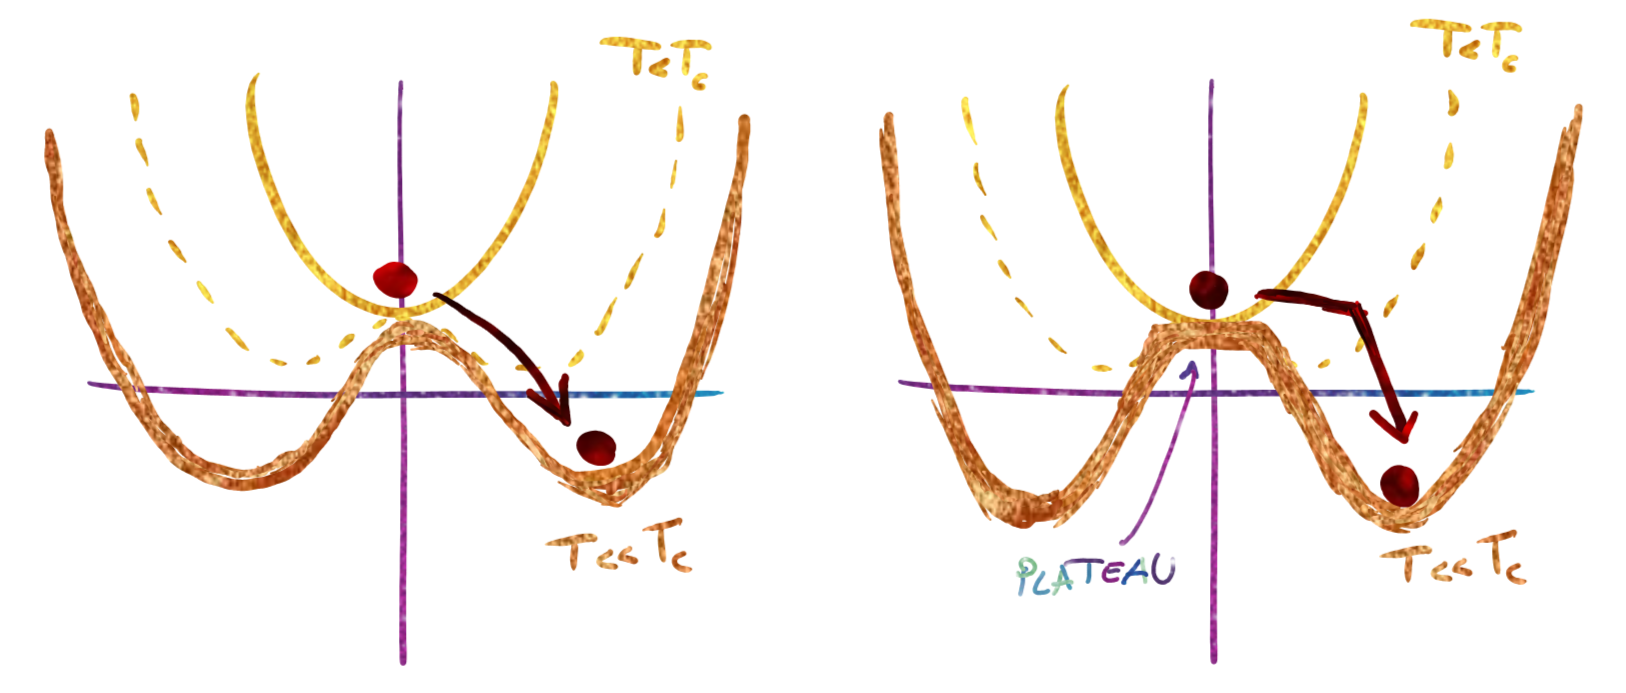
\includegraphics[width=.8\textwidth]{Pictures/4/transfase.png}
    \caption{Transizioni di fase del secondo (sinistra) e primo (destra) ordine o tipo.}
    \label{fig:4}
\end{figure}


\vspace{2em}
\noindent Le transizioni di fase che ha vissuto il nostro universo sono cronologicamente:
\begin{itemize}
    \item \textbf{GUT}: disaccoppiamento forza elettrodebole (leptoni) e forza forte (adroni). Questa è la transizione che più di tutte "svuota il vuoto" e avviene a ($10^{15 }$ GeV);
    \item \textbf{EWT}: disaccoppiamento forza debole e forza elettromagnetica ($10^{2}$ GeV);
    \item \textbf{QAT}: transizione quark-adrone ($0.2 \div 3$ GeV).
\end{itemize}
Inoltre, la teoria delle supersimmetrie prevederebbe un'ulteriore transizione di fase la cui scala è ancora oggetto di studio. 

Le condizioni di esistenza di una particella sono legate alla relazione:
$$
mc^2 = k_B T
$$
al passare del tempo $T$ diminuisce e, a causa di annichilazioni, sopravvivono soltanto particelle di massa via via minore e il loro livello di interazione è descritto da una sezione d'urto via via differente. L'equilibrio termico sarà raggiunto ogni qualvolta $\tau_{coll}\ll H^{-1}$ e questo è verificato sicuramente nellefasi primordiali poiché la materia è relativistica. Quando la condizione di equilibrio è verificata si può scrivere:

\begin{equation}
    n_i = \frac{g_i}{2\pi^2}\left ( \frac{k_B T}{\hslash c} \right )\int \frac{x^2 \mathrm{d}x}{e^x \pm 1} = \binom{3/4}{1} \frac{g_i}{\pi^2}~\xi (3)~T^3
\end{equation}
dove $g_i$ rappresenta il peso statistico della particella $i$-esima, $\xi (3) \approx 1.2$ e i valori $\pm$ e soprasotto si applicano rispettivamente alle particelle di tipo fermionico e bosonico. Per la densità di energia si ha:
\begin{equation}
    \rho_i c^2= \binom{7/8}{1} \frac{g_i}{2}~\sigma ~T^4
\end{equation}
Questa relazione può essere utilizzata per descrivere il fluido primordiale introducendo il peso statistico effettivo $g^*$, che descrive tutte le particelle accoppiate alla radiazione:
\begin{equation}
    \rho(T)c^2 = g^* ~ \frac{\sigma ~ T^2}{2} \qquad g^* = \sum g_{iB} + \frac{7}{8} \sum g_{iF} \label{eq:statisticweight}
\end{equation}
Oggi non c'è nulla accoppiato alla radiazione: $g^*=2$ (bosoni), in passato $g^*>2$. Per valutare l'equilibrio potrebbe essere necessario includere altri contributi alla densità (e.g. $\rho_{decoup}$, $\rho_{not\, rel}$, $\rho_{nt}$), che sono però trascurabili nelle fasi iniziali.